%%%%%%%%%%%%%%%%%%%%%%%%%%%%%%%%%%%%%%%%%%%%%%%%%%%%%%%%%%%%%%%%%%%%%%%%%%%%%%%%%%
 \begin{frame}[fragile]\frametitle{}
\begin{center}
{\Large Optimization }
\end{center}
\end{frame}

%%%%%%%%%%%%%%%%%%%%%%%%%%%%%%%%%%%%%%%%%%%%%%%%%%%%%%%%%%%%%%%%%%%%%%%%
\begin{frame}[fragile]\frametitle{Optimization}

\begin{itemize}
\item  Goal of Machine Learning is Optimization
\item Trying to find the`` best'' model for prediction
\item The ``best'' means that which minimizes prediction error.
\item The technique, widely used is called as ``Gradient Descent''
\end{itemize}
\end{frame}

%%%%%%%%%%%%%%%%%%%%%%%%%%%%%%%%%%%%%%%%%%%%%%%%%%%%%%%%%%%%%%%%%%%%%%%%
\begin{frame}[fragile]\frametitle{Example}

Trying to find relation (formula/model) between input x and output y

	\begin{table}[!h]
		\centering
		\begin{tabular}{| l | l |}
			\hline
			x & y \\ \hline
			2 & 4 \\ \hline
			6 & 12 \\ \hline
			3 & 7 \\ \hline
			4 & 7 \\ \hline
			12 & 24 \\ \hline
			21 & 40 \\ \hline			
		\end{tabular}
\end{table}
Any guesses?
\end{frame}

%%%%%%%%%%%%%%%%%%%%%%%%%%%%%%%%%%%%%%%%%%%%%%%%%%%%%%%%%%%%%%%%%%%%%%%%
\begin{frame}[fragile]\frametitle{Example}

How do you even start?

Assume $ y = w.x$ 

	\begin{table}[!h]
		\centering
		\begin{tabular}{| l | l |}
			\hline
			x & y \\ \hline
			2 & 4 \\ \hline
			6 & 12 \\ \hline
			3 & 7 \\ \hline
			4 & 7 \\ \hline
			12 & 24 \\ \hline
			21 & 40 \\ \hline			
		\end{tabular}
\end{table}

Now, how to find $w$?

\end{frame}

%%%%%%%%%%%%%%%%%%%%%%%%%%%%%%%%%%%%%%%%%%%%%%%%%%%%%%%%%%%%%%%%%%%%%%%%
\begin{frame}[fragile]\frametitle{Example}

Assume random value, say $w = 1$.

Using the relation, predict y, called y'

	\begin{table}[!h]
		\centering
		\begin{tabular}{| l | l | l|}
			\hline
			x & y & y'\\ \hline
			2 & 4  & 2\\ \hline
			6 & 12 & 6\\ \hline
			3 & 7  & 3\\ \hline
			4 & 7 & 4\\ \hline
			12 & 24 & 12\\ \hline
			21 & 40 & 21\\ \hline			
		\end{tabular}
\end{table}

Is y' matching actual y? NO. What to do? Need to find such $w$ for which both match, right?

\end{frame}

%%%%%%%%%%%%%%%%%%%%%%%%%%%%%%%%%%%%%%%%%%%%%%%%%%%%%%%%%%%%%%%%%%%%%%%%
\begin{frame}[fragile]\frametitle{Example}

How much OFF we are?

	\begin{table}[!h]
		\centering
		\begin{tabular}{| l | l | l| l|}
			\hline
			x & y & y' & y - y'\\ \hline
			2 & 4  & 2 & 2\\ \hline
			6 & 12 & 6 & 6\\ \hline
			3 & 7  & 3 & 4\\ \hline
			4 & 7 & 4 & 3\\ \hline
			12 & 24 & 12 & 12\\ \hline
			21 & 40 & 21 & 19 \\ \hline			
		\end{tabular}
\end{table}

Too much of diff. Summation of squares (to nullify effect of sign) will give total error. Huge!!

Lets try another value for $w$ and see if that works.

\end{frame}

%%%%%%%%%%%%%%%%%%%%%%%%%%%%%%%%%%%%%%%%%%%%%%%%%%%%%%%%%%%%%%%%%%%%%%%%
\begin{frame}[fragile]\frametitle{Example}

Lets try  $w = 0.5$.

Using the relation, and new $w$ predict y find the error again

	\begin{table}[!h]
		\centering
		\begin{tabular}{| l | l | l| l|}
			\hline
			x & y & y' & y - y'\\ \hline
			2 & 4  & \\ \hline
			6 & 12 & \\ \hline
			3 & 7  & \\ \hline
			4 & 7 & \\ \hline
			12 & 24 & \\ \hline
			21 & 40 & \\ \hline			
		\end{tabular}
\end{table}

Error going up or down? UP too much. So out ``direction'' of change was not good. Instead of reducing $w$ to 0.5, we should try increasing it to 1.5.

\end{frame}


%%%%%%%%%%%%%%%%%%%%%%%%%%%%%%%%%%%%%%%%%%%%%%%%%%%%%%%%%%%%%%%%%%%%%%%%
\begin{frame}[fragile]\frametitle{Example}

Lets try  $w = 1.5$.

Using the relation, and new $w$ predict y find the error again

	\begin{table}[!h]
		\centering
		\begin{tabular}{| l | l | l| l|}
			\hline
			x & y & y' & y - y'\\ \hline
			2 & 4  & \\ \hline
			6 & 12 & \\ \hline
			3 & 7  & \\ \hline
			4 & 7 & \\ \hline
			12 & 24 & \\ \hline
			21 & 40 & \\ \hline			
		\end{tabular}
\end{table}

Error going up or down? Better. So out ``direction'' of change good but still error does not seem to close to 0. Increase $w$ further.

\end{frame}

%%%%%%%%%%%%%%%%%%%%%%%%%%%%%%%%%%%%%%%%%%%%%%%%%%%%%%%%%%%%%%%%%%%%%%%%
\begin{frame}[fragile]\frametitle{Example}

Lets try  $w = 2$.

Using the relation, and new $w$ predict y find the error again

	\begin{table}[!h]
		\centering
		\begin{tabular}{| l | l | l| l|}
			\hline
			x & y & y' & y - y'\\ \hline
			2 & 4  & \\ \hline
			6 & 12 & \\ \hline
			3 & 7  & \\ \hline
			4 & 7 & \\ \hline
			12 & 24 & \\ \hline
			21 & 40 & \\ \hline			
		\end{tabular}
\end{table}

Looks far better. Best? Probably. So relation now is $y = 2.x$. Seems to be correct for all rows except 1 or 2. But thats ok.

\end{frame}

%%%%%%%%%%%%%%%%%%%%%%%%%%%%%%%%%%%%%%%%%%%%%%%%%%%%%%%%%%%%%%%%%%%%%%%%
\begin{frame}[fragile]\frametitle{Maximization Minimization}
\begin{itemize}
\item  Ideas is to minimize the differences, also called as Error, Loss, Cost.
\item It depends on $w$
\item So, this is a minimzation problem of Cost wrt w
\item How do you find minimum of ANY function?
\end{itemize}
\end{frame}


%%%%%%%%%%%%%%%%%%%%%%%%%%%%%%%%%%%%%%%%%%%%%%%%%%%%%%%%%%%%%%%%%%%%%%%%
\begin{frame}[fragile]\frametitle{Maximization Minimization}
\begin{itemize}
\item  Suppose we have a function $f$ taking vector (or list of values) and outputs a single number.
\item We frequently need to maximize or minimize the the function.
\item Meaning, we wish to try many input vectors and find one where the result is minimum or maximum
\item Examples: minimize cost of operations, maximize profits, etc.
\end{itemize}
\end{frame}

%%%%%%%%%%%%%%%%%%%%%%%%%%%%%%%%%%%%%%%%%%%%%%%%%%%%%%%%%%%%%%%%%%%%%%%%
\begin{frame}[fragile]\frametitle{Example}
Say, our function is $\sum x_i ^2$
\begin{lstlisting}
def sum_of_squares(v):
	"""computes	the sum of squared elements in v"""
	return	sum(v_i**2 for v_i in v)
\end{lstlisting}
\begin{itemize}
\item Let's use gradients to find the minimum among all three-dimensional vectors
\item We'll just pick a random starting point 
\item Take tiny steps in the opposite direction of the gradient 
\item Until we reach a point where the gradient is very small.
\end{itemize}
\end{frame}

%%%%%%%%%%%%%%%%%%%%%%%%%%%%%%%%%%%%%%%%%%%%%%%%%%%%%%%%%%%%%%%%%%%%%%%%
\begin{frame}[fragile]\frametitle{Example}
\begin{center}
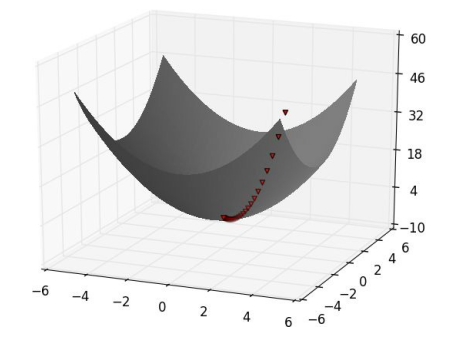
\includegraphics[width=0.8\linewidth]{graddesc}
\end{center}
\end{frame}

%%%%%%%%%%%%%%%%%%%%%%%%%%%%%%%%%%%%%%%%%%%%%%%%%%%%%%%%%%%%%%%%%%%%%%%%
\begin{frame}[fragile]\frametitle{Example}
Random vector, starting point
\begin{lstlisting}
v = [random.randint(-10,10) for	i in range(3)]
\end{lstlisting}
Our Gradient function is, derivative of $\sum x_i ^2$ which is $\sum 2 x_i$
\begin{lstlisting}
def sum_of_squares_gradient(v):
	return	[2 * v_i for v_i in v]
\end{lstlisting}
\end{frame}

%%%%%%%%%%%%%%%%%%%%%%%%%%%%%%%%%%%%%%%%%%%%%%%%%%%%%%%%%%%%%%%%%%%%%%%%
\begin{frame}[fragile]\frametitle{Example}
Step is computed as below, if size is -ve then its in opposite of gradient.
\begin{lstlisting}
def step(v, direction, step_size):
	"""move step_size in the direction from v"""
	return	[v_i - step_size * direction_i for v_i, direction_i in zip(v, direction)]
\end{lstlisting}
\end{frame}

%%%%%%%%%%%%%%%%%%%%%%%%%%%%%%%%%%%%%%%%%%%%%%%%%%%%%%%%%%%%%%%%%%%%%%%%
\begin{frame}[fragile]\frametitle{Example}
Core logic:
\begin{lstlisting}
tolerance = 0.0000001
while True:
	gradient = sum_of_squares_gradient(v) 
	next_v = step(v, gradient, 0.01) 
	if gradient < tolerance: 
		break
	v = next_v																			
\end{lstlisting}
We end-up at $[0,0,0]$ which is obvious.
\end{frame}

%%%%%%%%%%%%%%%%%%%%%%%%%%%%%%%%%%%%%%%%%%%%%%%%%%%%%%%%%%%%%%%%%%%%%%%%
\begin{frame}[fragile]\frametitle{Considerations}
\begin{itemize}
\item Choosing the right step size is critical
\item Using fixed step size
\item Gradually shrinking step size
\end{itemize}
\end{frame}


%%%%%%%%%%%%%%%%%%%%%%%%%%%%%%%%%%%%%%%%%%%%%%%%%%%%%%%%%%%%%%%%%%%%%%%%
\begin{frame}[fragile]\frametitle{Learning rate is too small}
\begin{center}
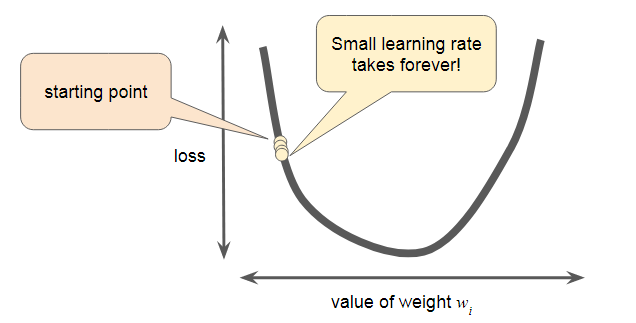
\includegraphics[width=0.8\linewidth]{lr1}
\end{center}


\tiny{(Reference:https://developers.google.com/machine-learning/crash-course/reducing-loss/learning-rate)}
\end{frame}

%%%%%%%%%%%%%%%%%%%%%%%%%%%%%%%%%%%%%%%%%%%%%%%%%%%%%%%%%%%%%%%%%%%%%%%%
\begin{frame}[fragile]\frametitle{Learning rate is too large}
\begin{center}
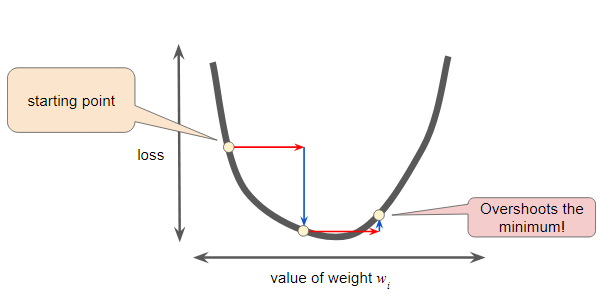
\includegraphics[width=0.8\linewidth]{lr2}
\end{center}


\tiny{(Reference:https://developers.google.com/machine-learning/crash-course/reducing-loss/learning-rate)}
\end{frame}

%%%%%%%%%%%%%%%%%%%%%%%%%%%%%%%%%%%%%%%%%%%%%%%%%%%%%%%%%%%%%%%%%%%%%%%%
\begin{frame}[fragile]\frametitle{ Learning rate is just right}

The Goldilocks value is related to how flat the loss function is. If you know the gradient of the loss function is small then you can safely try a larger learning rate, which compensates for the small gradient and results in a larger step size.


\begin{center}
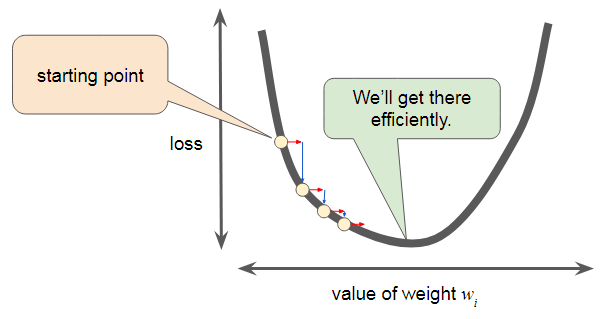
\includegraphics[width=0.8\linewidth]{lr3}
\end{center}


\tiny{(Reference:https://developers.google.com/machine-learning/crash-course/reducing-loss/learning-rate)}
\end{frame}


%%%%%%%%%%%%%%%%%%%%%%%%%%%%%%%%%%%%%%%%%%%%%%%%%%%%%%%%%%%%%%%%%%%%%%%%%%
%%\begin{frame}[fragile]\frametitle{Line fitting on real data}
%%\begin{center}
%%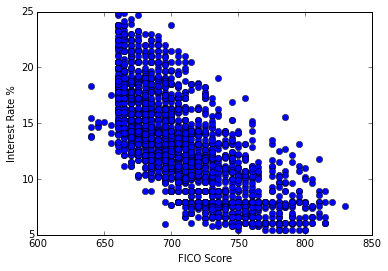
\includegraphics[width=0.5\linewidth]{loan1}
%%\end{center}
%%\begin{itemize}
%%\item Here we see a distinct downward linear trend where Interest Rate goes down with increasing FICO score. 
%%\item But we also see that for the same FICO score there is a range of Interest rates.
%%\item This suggests that FICO by itself might not be enough to predict Interest Rate.
%%\end{itemize}
%%\end{frame}
%%
%%
%%%%%%%%%%%%%%%%%%%%%%%%%%%%%%%%%%%%%%%%%%%%%%%%%%%%%%%%%%%%%%%%%%%%%%%%%%
%%\begin{frame}[fragile]\frametitle{Line fitting on real data}
%%The Lending Club is a peer-to-peer lending site where members make loans to each other. The site makes anonymized data on loans and borrowers publicly available.
%%Just look at how borrower FICO score affects interest rate charged.
%%\begin{lstlisting}
%%import pandas as pd
%%df = pd.read_csv('../datasets/loanf.csv')
%%
%%intrate = df['Interest.Rate']
%%fico = df['FICO.Score']
%%p = plot(fico,intrate,'o')
%%ax = gca()
%%xt = ax.set_xlabel('FICO Score')
%%yt = ax.set_ylabel('Interest Rate %')
%%\end{lstlisting}
%%\end{frame}
